\documentclass[aspectratio=169]{beamer}

\usepackage{tikz}
\usepackage{caption}
\usepackage{colortbl}
\usepackage{qrcode}
\usepackage{hyperref}
\setbeamertemplate{caption}[numbered]
\setbeamertemplate{section in toc}[sections numbered]
\newbool{russian}
\booltrue{russian}  % Загружает русскоязычный логотип
\usepackage{theme/theme} % Подгружаем тему

%%% Работа с русским языком и шрифтами
\usepackage[english,russian]{babel}   % загружает пакет многоязыковой вёрстки
\usepackage[no-math]{fontspec}      % подготавливает загрузку шрифтов Open Type, True Type и др.
	\setsansfont{Liberation Sans} 
	\setmonofont{Courier New}
\usepackage{mathspec}
	\setmathsfont(Digits,Latin,Greek)[Numbers={Lining,Proportional}]{Liberation Sans}
	\setmathrm[Numbers={Lining,Proportional}]{Liberation Sans}
\uselanguage{russian}
\languagepath{russian}
\graphicspath{{images/}}  	% Папка с картинками

%%% Информация об авторе и выступлении
\title[Заголовок]{Издательская система \LaTeX{}} 
\subtitle{Статьи, ссылки, системы контроля версий}
\author[Имя автора]{Александр Сергеевич Филипченко \\ \smallskip \scriptsize 797439@edu.rut-miit.ru\\}
\institute{кафедра <<Вычислительные системы, сети и информационная безопасность>>}

\begin{document}	% Начало презентации

\frame[plain]{\titlepage}	% Титульный слайд

\begin{frame}
\frametitle{План лекции}
\tableofcontents
\end{frame}

\section{Особенности подготовки научных статей в \LaTeX{}}

\begin{frame}
\frametitle{Библигорафия. Программный пакет BibLaTeX}
BibLaTeX --- менеджер библиографии.
Состоит из утилиты для работы с \texttt{.bib} файлами \textbf{biber} и пакета \textbf{biblatex}.
Алгоритм работы менеджера библиографии:
\begin{enumerate} 
\item программа \textbf{xelatex} обнаруживает ссылки (команды \texttt{\textbf{\textbackslash cite}}) и подключенные источники в формате в документе и по результатам формирует запрос;
\item программа \textbf{biber} формирует в ответ на запрос LaTeX-файл с нужными библиографическими данными;
\item программа \textbf{xelatex} выполняет проход для расстановки ссылок и добавления списка литературы в документ;
\item программа \textbf{xelatex} выполняет дополнительный проход для перерасстановки номеров страниц и внутренних ссылок в документе.
\end{enumerate} 
\end{frame}

\begin{frame}
\frametitle{Пример использования BibLaTeX}
\medskip
\begin{columns}
\column{0.5\textwidth}
\begin{figure}
\centering
\begin{tikzpicture}
\node[draw=black, line width=1pt, inner sep=0pt] {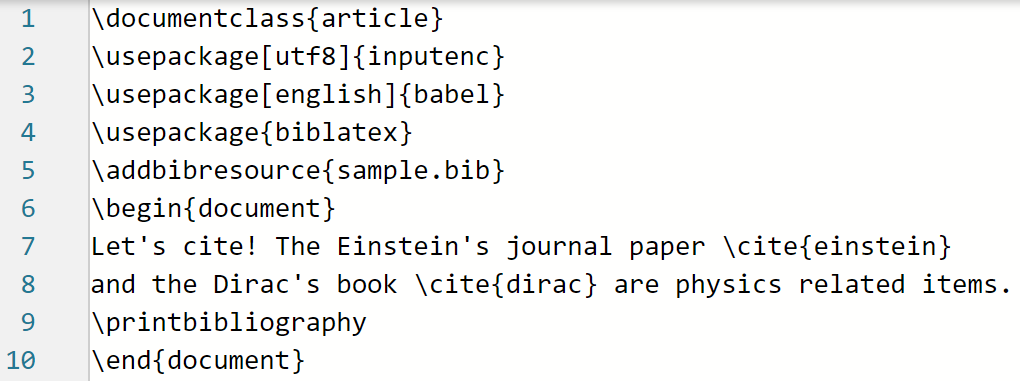
\includegraphics[width=\columnwidth]{BibLatexCode}};
\end{tikzpicture}
\caption{Пример исходного кода с использованием BibLaTeX}
\end{figure}
\column{0.5\textwidth}
\begin{figure}
\centering
\begin{tikzpicture}
\node[draw=black, line width=1pt, inner sep=0pt] {
\includegraphics[width=\columnwidth]{BibLatexRes}};
\end{tikzpicture}
\caption{Результат сборки}
\end{figure}
\end{columns}
\end{frame}

\begin{frame}
\frametitle{Способы управления библиографией}
Выбор стиля осуществляется через параметр \texttt{style=stylename} при вызове \texttt{\textbf{\textbackslash usepackage}}).
Параметр \texttt{sorting=option} определяет критерий сортировки источников в библиографическом списке.
\begin{table}[]
	\begin{tabular}{ll}
\textbf{опция} & \textbf{характеристика}                   \\ \hline
nty            & сортировка по имени, названию, году       \\
nyt            & сортировка по имени, году, названию       \\
nyvt           & сортировка по имени, году, тому, названию \\
...            & и иные комбинации этих букв               \\
none           & сортировка по порядку цитирования        
\end{tabular}
\end{table}
\end{frame}

\begin{frame}
\frametitle{Подготовка библиографического файла}
При подготовке библиографического файла \texttt{.bib} в BibLaTeX существует несколько типов записей, каждый из которых имеет свои специфические параметры.
\begin{table}[]
	\begin{tabular}{ll}
\textbf{Тип записи} & \textbf{Характеристика} \\ \hline
@book       & Книга \\
@article    & Статья в журнале \\
@conference & Материалы конференции \\
@thesis     & Диссертация или дипломная работа \\
@report     & Технический отчет \\
@manual     & Руководство или инструкция \\
@misc       & Разное (для записей, которые не подходят под другие категории)
\end{tabular}
\end{table}
\end{frame}

\begin{frame}
\frametitle{Примеры записей в библиографическом файле}
\medskip
\begin{columns}
\column{0.5\textwidth}
\begin{figure}
\centering
\begin{tikzpicture}
\node[draw=black, line width=1pt, inner sep=0pt] {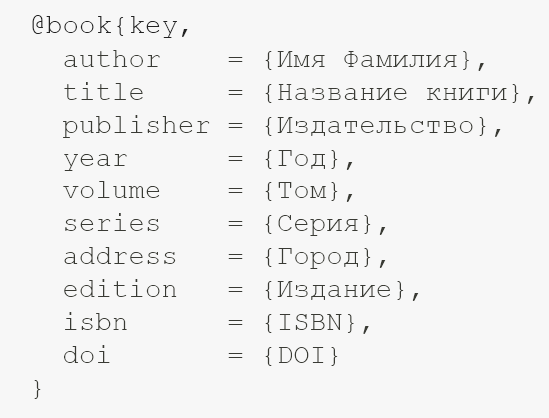
\includegraphics[width=\columnwidth]{bibBook}};
\end{tikzpicture}
\caption{Параметры библиографического описания типа <<Книга>>}
\end{figure}
\column{0.5\textwidth}
\begin{figure}
\centering
\begin{tikzpicture}
\node[draw=black, line width=1pt, inner sep=0pt] {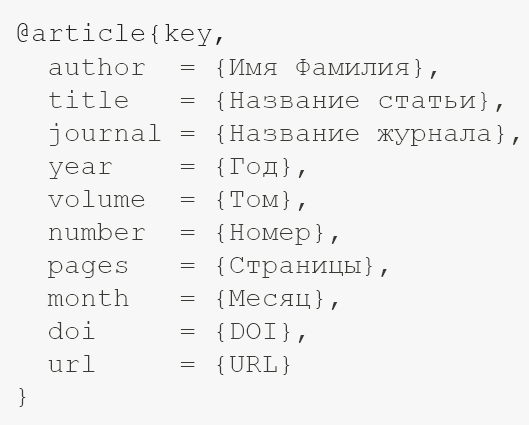
\includegraphics[width=\columnwidth]{bibArticle}};
\end{tikzpicture}
\caption{Параметры <<Статьи>>}
\end{figure}
\end{columns}
\end{frame}

\begin{frame}
\frametitle{Работа с изображениями}
\LaTeX{} не может самостоятельно управлять изображениями, поэтому необходимо использовать пакет \textbf{graphicx}.
\begin{exampleblock}{Каталог изображений}
Команда \texttt{\textbf{\textbackslash graphicspath}} сообщает \LaTeX{}, что изображения хранятся в каталоге, имя которого передано в качестве параметра.
\end{exampleblock}
\begin{exampleblock}{Включение изображения}
Команда \texttt{\textbf{\textbackslash includegraphics}} непосредственно включает изображение в документ.
В качестве параметра ей передаётся имя файла с изображением без расширения.
Имя файла с изображением не должно содержать пробелов и многоточий.
\end{exampleblock}
\end{frame}

\begin{frame}
\frametitle{Картинки}
\begin{exampleblock}{Позиционирование}
Управлять размерами изобращений можно при помощи параметров \textbf{scale}, \textbf{width}, \textbf{height}.
Вместо конкретных численных значений ширины можно, например, задавать размер по ширине текста через \texttt{\textbf{width = \textbackslash textwidth}}.
\end{exampleblock}
\begin{exampleblock}{Подписи}
Подписи добавляющие краткое описание к изображениям.
Вызываются командой \texttt{\textbf{\textbackslash caption}}, которой в качестве параметра передаётся непсоредственно сам текст подписи.
Подписи также поддреживают автонумерацию.
\end{exampleblock}
\end{frame}

\section{Ссылки на элементы документа}

\begin{frame}
\frametitle{Метки}
В \LaTeX{} мы можем помечать нумерованные объекты (разделы, формулы и т. д.), а затем использовать эту метку для ссылки на них в других местах.
Те же команды применимы и к окружению рисунков.
Оперирует тремя основными компонентами:
\begin{itemize}
\item \texttt{\textbf{\textbackslash label\{marker\}}} --- маркер можно рассматривать как имя, которое мы даем объекту, на который хотим сослаться. Важно добавить \label после нумерованного элемента, например, иначе метка не сможет «зацепиться» за нужный номер или счетчик.
\item \texttt{\textbf{\textbackslash ref\{marker\}}} --- выводит номер, присвоенный объекту, помеченному маркером.
\item \texttt{\textbf{\textbackslash pageref\{marker\}}} --- выводит номер страницы, на которой появился объект, помеченный маркером.
\end{itemize}
\end{frame}

\begin{frame}
\frametitle{Пример}
\medskip
\begin{columns}
\column{0.5\textwidth}
\begin{figure}
\centering
\begin{tikzpicture}
\node[draw=black, line width=1pt, inner sep=0pt] {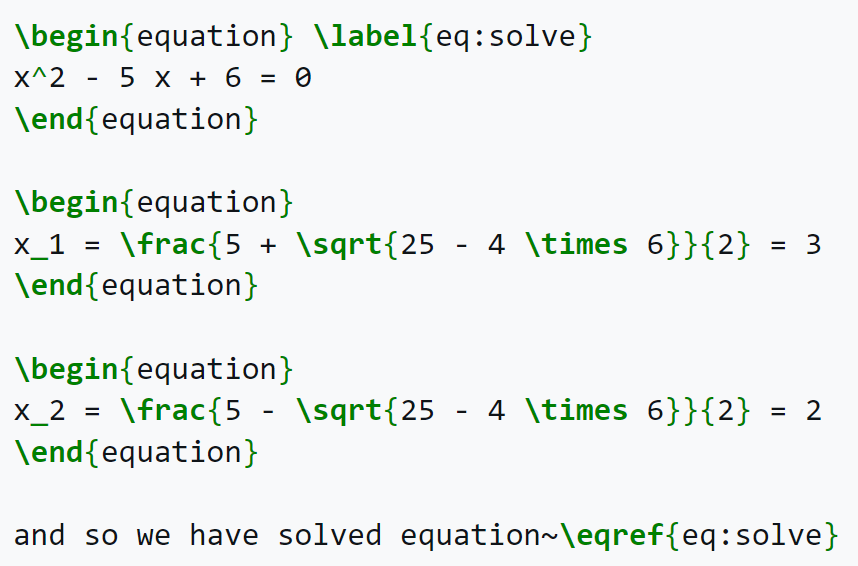
\includegraphics[width=\columnwidth]{labelCode}};
\end{tikzpicture}
\caption{Ссылаемся на первую формулу}
\end{figure}
\column{0.5\textwidth}
\begin{figure}
\centering
\begin{tikzpicture}
\node[draw=black, line width=1pt, inner sep=0pt] {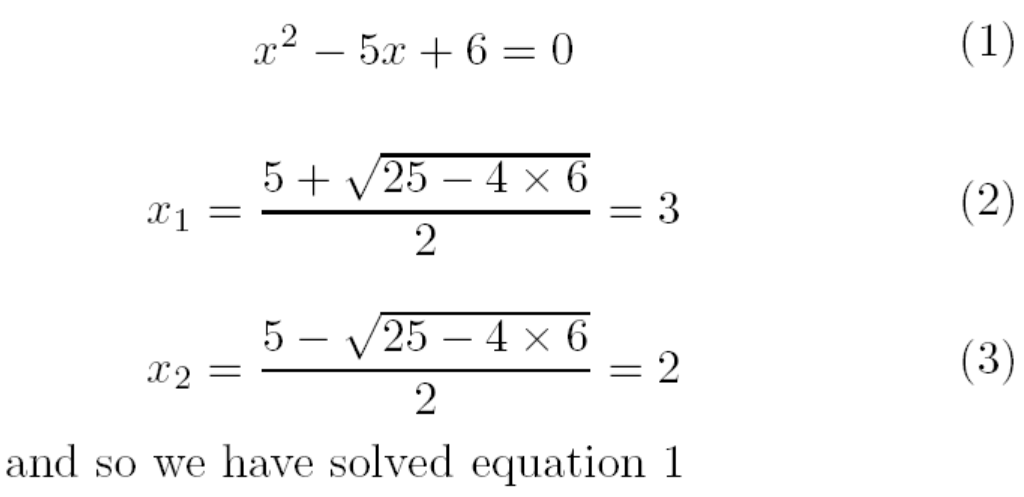
\includegraphics[width=\columnwidth]{labelRes}};
\end{tikzpicture}
\caption{Результат сборки}
\end{figure}
\end{columns}
\end{frame}

\section{Использование системы контроля версий}

\begin{frame}
\frametitle{Системы контроля версий}
Системы контроля версий --- специализированное программное обеспечение, предназначенное для синхронизации актуальных версий файлов и документов между рабочими местами участников проекта, ведение истории изменений.
\begin{exampleblock}{Преимущества}
\begin{itemize}
\item \textbf{Отслеживание изменений}. СКВ позволяет фиксировать каждое изменение в файлах, что дает возможность вернуться к предыдущим версиям при необходимости. Это особенно полезно, если что-то пошло не так.
\item \textbf{Совместная работа}. Несколько разработчиков могут работать над одним проектом одновременно, не опасаясь конфликтов. СКВ помогает объединять изменения и разрешать конфликты, если они возникают.
\end{itemize}
\end{exampleblock}
\end{frame}

\begin{frame}
\frametitle{Преимущества СКВ}
\begin{exampleblock}{Преимущества}
\begin{itemize}
\item \textbf{История изменений}. СКВ сохраняет полную историю изменений, включая информацию о том, кто и когда вносил изменения. Это позволяет легко отслеживать, когда и почему были сделаны определенные изменения.
\item \textbf{Безопасность}. СКВ обеспечивает резервное копирование данных. Если файл был случайно удален или поврежден, его можно восстановить из предыдущей версии.
\item \textbf{Управление версиями}. СКВ позволяет создавать разные ветки разработки, что дает возможность экспериментировать с новыми функциями или исправлениями, не влияя на основную версию проекта.
\end{itemize}
\end{exampleblock}
\end{frame}

\begin{frame}
\frametitle{Терминология СКВ}
\begin{alertblock}{Репозиторий}
Место, где хранятся все файлы проекта и их история изменений. Репозиторий может быть локальным (на вашем компьютере) или удаленным (на сервере).
\end{alertblock}
\begin{alertblock}{Коммит}
Фиксация изменений в репозитории. Каждый коммит содержит информацию о том, какие изменения были внесены, кто их сделал и когда.
\end{alertblock}
\begin{alertblock}{Ветка}
Отдельная линия разработки, которая позволяет работать над новыми функциями или исправлениями, не влияя на основную (главную) версию проекта. Ветки позволяют параллельно разрабатывать разные версии проекта.
\end{alertblock}
\begin{alertblock}{Слияние}
Процесс объединения изменений из одной ветки в другую.
\end{alertblock}
\end{frame}

\begin{frame}
\frametitle{Терминология СКВ}
\begin{alertblock}{Конфликт}
Ситуация, когда изменения в разных ветках затрагивают одни и те же строки кода, и система не может автоматически определить, какие изменения следует сохранить.
\end{alertblock}
\begin{alertblock}{Тег}
Метка, которая используется для обозначения конкретной версии или состояния проекта. Теги часто используются для обозначения релизов.
\end{alertblock}
\begin{alertblock}{Клонирование}
Процесс создания локальной копии удаленного репозитория. Это позволяет пользователям работать с проектом на своем компьютере.
\end{alertblock}
\begin{alertblock}{Форк}
Копия репозитория, созданная для внесения изменений, которая может быть предложена для слияния обратно в оригинальный репозиторий.
\end{alertblock}
\end{frame}

\begin{frame}
\frametitle{Пример}
\medskip
\begin{columns}
\column{0.5\textwidth}
Пример графа истории проекта с контролем ревизий; ствол --- зелёный, ветви --- жёлтый, а граф не является деревом из-за наличия слияний (красные стрелки).
\column{0.5\textwidth}
\begin{figure}
\centering
\begin{tikzpicture}
\node[draw=black, line width=1pt, inner sep=0pt] {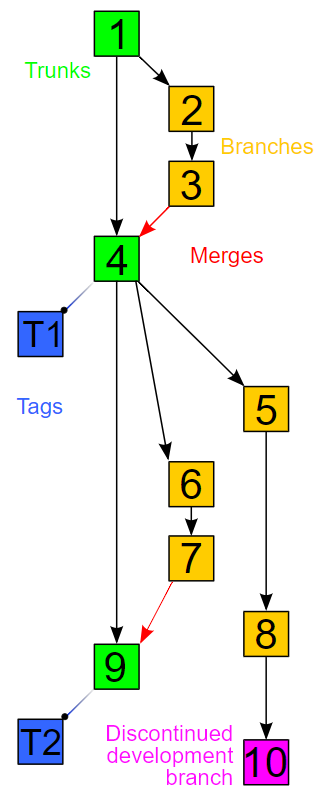
\includegraphics[scale=0.25]{vcsEx}};
\end{tikzpicture}
\end{figure}
\end{columns}
\end{frame}

\begin{frame}
\frametitle{Основные команды СКВ \textbf{git}}
\begin{alertblock}{git init}
Создает новый локальный репозиторий в текущей директории.
\end{alertblock}
\begin{alertblock}{git clone \textit{url}}
Клонирует удаленный репозиторий на локальный компьютер.
\end{alertblock}
\begin{alertblock}{git add \textit{filename}}
Добавляет изменения в указанных файлах в индекс для последующего коммита.
\end{alertblock}
\begin{alertblock}{git commit -m "message"}
Фиксирует изменения в индексе с сообщением о коммите.
\end{alertblock}
\end{frame}

\begin{frame}
\frametitle{Команды для работы с ветками}
\begin{alertblock}{git branch}
Показывает список всех веток в репозитории. Если указать имя ветки, команда создаст новую ветку.
\end{alertblock}
\begin{alertblock}{git checkout \textit{branch}}
Переключает на указанную ветку.
\end{alertblock}
\begin{alertblock}{git merge \textit{branch}}
Объединяет изменения из указанной ветки в текущую ветку.
\end{alertblock}
\end{frame}

\begin{frame}
\frametitle{Команды для работы с удаленными репозиториями}
\begin{alertblock}{git remote}
Показывает список удаленных репозиториев. Можно использовать с параметрами для добавления, удаления или изменения удаленных репозиториев.
\end{alertblock}
\begin{alertblock}{git push \textit{remote} \textit{branch}}
Отправляет изменения из локальной ветки в удаленный репозиторий.
\end{alertblock}
\begin{alertblock}{git pull \textit{remote} \textit{branch}}
Загружает изменения из удаленного репозитория и объединяет их с текущей веткой.
\end{alertblock}
\end{frame}

\begin{frame}
\frametitle{Пример проекта в СКВ}
\medskip
\begin{columns}
\column{0.5\textwidth}
Данная презентация подготовлена с использованием СКВ \textbf{git}. Справа приведена ссылка на соответсвующий репозиторий на платформе <<GitHub>>.
\column{0.5\textwidth}
\qrset{link, height=3cm}
\qrcode{https://github.com/mrtree4/RUT-MIIT-beamer}
\end{columns}
\end{frame}

\section{Домашнее задание}

\begin{frame}
\frametitle{Подготовка доклада}
На основе созданного шаблона написать доклад про архитектуру 16-разрядных микропроцессоров Intel 8086.
\begin{exampleblock}{Требования}
\begin{itemize}
\item использовать систему контроля версий;
\item объём от 10 страниц;
\item использовать источники с портала eLibary и Киберленинка;
\item сортировать список использованных источников по фамилиям авторов;
\item должны быть формулы, таблицы и картинки.
\end{itemize}
\end{exampleblock}
\end{frame}

\end{document}
